\section{Introdução}
Atualmente, a aplicação de grafos vem sendo cada vez mais utilizada no mundo da computação, por ser bastante versatil na resolução de problemas. Um exemplo é o aplicativo Waze, que utiliza grafos para traçar o caminho a ser percorrido de um ponto a outro. Pode-se observar com isso, que a descoberta de caminhos disjuntos teria uma boa função nesse aplicativo, pois permitiria que o motorista que não queira utilizar o caminho inicial disponibilizado pelo aplicativo, possa solicitar um novo. Assim, utilizando o método proposto neste trabalho, é possível realizar uma busca para descobrir caminhos diferente para o usuário, caso exista algum..

\section{Desenvolvimento}

\subsection{Entrada de dados}
Para a entrada de dados, foi utilizada a linha de comando para passar os argumentos, que são respectivamente: o arquivo contendo o grafo criado ou nome do arquivo que deseja criar o grafo; o vértice de origem para a busca dos caminhos; o vértice de destino para a busca chegar até ele.

A partir disso, para criar um grafo, basta fazer um arquivo \emph{.txt} passando na primeira linha, a quantidade de vértices, e a lista de arestas nas próximas linhas, da seguinte forma \emph{vértice\_saída vértice\_entrada}, onde vértice de saída é de onde a aresta sai e o vértice de entrada e onde a aresta entra, mostrado na Figura \ref{fig:figure1}. Essa situação se encaixa caso o grafo que deseja seja diferente dos grafos de teste abordados na Seção \ref{sec:results} do artigo.

\begin{figure}[ht]
    \centering
    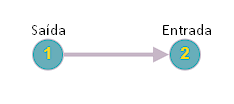
\includegraphics[width=.3\textwidth]{figuras/aresta_example.png}
    \caption{Exemplo de aresta direcionada}
    \label{fig:figure1}
\end{figure}

Com isso, ao passar por parâmetro o vértice de origem e o vértice de destino, eles serão utilizados para calcular o número máximo de caminhos disjuntos para o grafo desejado. Mostrando também todos os caminhos percorridos, utilizando os vértices passados, a Figura \ref{fig:figure2} exemplifica cada caminho disjunto em aresta, que é um caminho que sai de um vértice de destino até um vértice de origem sem repetir a aresta novamente.

\newpage

\begin{figure}[ht]
    \centering
    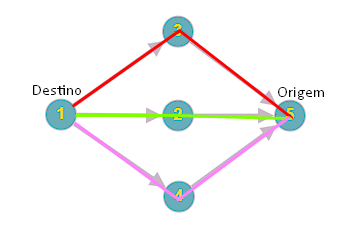
\includegraphics[width=.5\textwidth]{figuras/disjoint paths.png}
    \caption{Caminhos disjuntos em arestas em um grafo}
    \label{fig:figure2}
\end{figure}

\subsection{Descobrir caminhos disjuntos}

O algoritmo desenvolvido para encontrar a maior quantidade de caminhos possíveis em um grafos direcionado partindo de um vértices \(s\) e até um vértice \(t\) utilizando os \(n\) vértices do grafo.

O método executa uma busca em profundidade tentando encontrar o vértice \(t\). Ao encontrá-lo, o caminho utilizado é salvo e as arestas pertencentes a esse caminho são invertidas em um grafo auxiliar, ou seja, se ela era \((v,w)\) ela se torna \((w,v)\). Tal alteração parte da mesma ideia presente nos métodos de cálculo de fluxo máximo que é de consumir toda a capacidade da aresta e invertê-la. 

A cada caminho encontrado a variável responsável por contabilizar a quantidade de caminhos disjuntos é incrementada em 1. O método se repete até que mais nenhum caminho seja encontrado.

\begin{algorithm}[H]
\caption{Encontrar a maior quantidade possível de caminhos disjuntos em um grafo direcionado}
\begin{algorithmic}[1]
\REQUIRE $(origin \in n \land destiny \in\ n)$
\STATE $auxGraph \leftarrow copy(graph)$
\STATE $parent \leftarrow [ ]$
\STATE $maxPaths \leftarrow 0$
\STATE $paths \leftarrow NULL$
\WHILE{$auxGraph.search(origin, destiny, parent)$}
    \STATE $reversedPath \leftarrow NULL$
    \STATE $v \leftarrow destiny$
    \WHILE{$v \neq origin$}
        \STATE $u \leftarrow parent[v]$
        \STATE $reversedPath.append(v)$
        \STATE $auxGraph.removeEdge(u, v)$
        \STATE $auxGraph.addEdge(v, u)$
        \STATE $v \leftarrow parent[u]$
    \ENDWHILE
    \STATE $reversedPath.append(origin)$
    \STATE $path \leftarrow reversedPath.popAllElements()$
    \STATE $paths.append(path)$
    \STATE $maxPaths \leftarrow maxFlow + 1$
\ENDWHILE
\RETURN $maxPaths, paths$
\end{algorithmic}
\end{algorithm}

\section{Resultados e testes}
\label{sec:results}

Os testes foram feitos em 3 tipos diferentes de topologias, cada uma seguindo sua regra específica de formação, elas serão nomeadas como \emph{Topologia 1}, \emph{Topologia 2}, \emph{Topologia 3}. Além disso, cada topologia foi testada utilizando quantidades diferentes de vértices, sendo elas: 10, 100, 500, 1000 e 10.000.

\subsection{Topologia 1 - Grafo Circular}

A \emph{Topologia 1} segue a ideia padrão de um grafo cíclico, direcionado, não ponderado e sem arestas antiparalelas. Ele é formado por \emph{n} vértices e \emph{n} arestas.

\begin{figure}[hbt!]
    \centering
    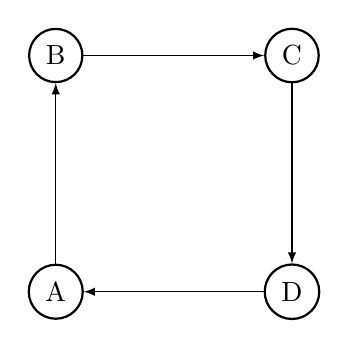
\begin{tikzpicture}[every node/.style={circle,thick,draw}]
        \tikzset{edge/.style = {->,> = latex}}
        \node (A) at (0,0) {A};
        \node (B) at (0,3) {B};
        \node (C) at (3,3) {C};
        \node (D) at (3,0) {D};
        
        \draw[edge] (A) to (B);
        \draw[edge] (B) to (C);
        \draw[edge] (C) to (D);
        \draw[edge] (D) to (A);
\end{tikzpicture} 
    \caption{Grafo cíclico sem arestas antiparalelas}
    \label{fig:my_label}
\end{figure}

\begin{algorithm}[H]
\caption{Gerar grafo circular}
\begin{algorithmic} 
\REQUIRE $n > 0$
\STATE $i \leftarrow 0$
\STATE $edges \leftarrow NULL$
\FOR{$i < n$}
\IF{$i \neq  (n-1)$}
\STATE $edges \mathrel{{+}{=}} (i, i + 1)$
\ENDIF
\ENDFOR
\STATE $edges \mathrel{{+}{=}} (n - 1, 0)$
\RETURN $edges$
\end{algorithmic}
\end{algorithm}

No algoritmo acima, o \emph{n} representa a quantidade de vértices desejado, ela deve ser maior do que 0. Já a variável \emph{edges} é formada por uma lista de tuplas, em cada tupla representa uma aresta \emph{(v,w)}, em que ela sai de \emph{v} e incide em \emph{w}.

\subsection{Topologia 2 - Grafo Simples}

A \emph{Topologia 2} baseia-se na ideia de possuir \emph{n} vértices, em que um vértice possui um grau de saída igual a \(n - 1\) e grau de entrada igual a 0 e um outro vértice que possui um grau de saída igual a 0 e um grau de entrada igual a \(n-1\). Na prática, a geração baseia-se em adicionar uma aresta \((v,w)\) para todo par de vértices em que \emph{v} preceda \emph{w} em um conjunto de vértices ordenado lexicograficamente.

\begin{figure}[hbt!]
    \centering
    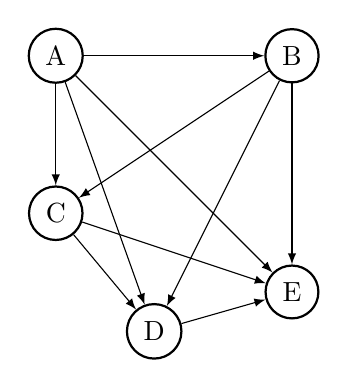
\begin{tikzpicture}[every node/.style={circle,thick,draw}]
        \tikzset{edge/.style = {->,> = latex}}
        \node (A) at (0,3) {A};
        \node (B) at (3,3) {B};
        \node (C) at (0,1) {C};
        \node (D) at (1.25,-0.5) {D};
        \node (E) at (3,0) {E};
        
        \draw[edge] (A) to (B);
        \draw[edge] (A) to (C);
        \draw[edge] (A) to (D);
        \draw[edge] (A) to (E);
        
        \draw[edge] (B) to (C);
        \draw[edge] (B) to (D);
        \draw[edge] (B) to (E);
        
        \draw[edge] (C) to (D);
        \draw[edge] (C) to (E);
        
        \draw[edge] (D) to (E);
\end{tikzpicture} 
    \caption{Grafo formado por 5 vértices seguindo regra específica de formação}
    \label{fig:my_label}
\end{figure}

\begin{algorithm}[H]
\caption{Gerar grafo com regra de formação específica}
\begin{algorithmic} 
\REQUIRE $n > 0$
\STATE $i \leftarrow 0$
\STATE $edges \leftarrow NULL$
\FOR{$i < n$}
\STATE{$j \leftarrow i$}
\FOR{$j < n$}
\IF{$i \neq j$}
\STATE $edges \mathrel{{+}{=}} (i, j)$
\ENDIF
\ENDFOR
\ENDFOR
\RETURN $edges$
\end{algorithmic}
\end{algorithm}

\subsection{Topologia 3 - Grafo Completo}
A terceira e última topologia, chamada de \emph{Topologia 3}, utiliza de dois \emph{K-n} grafos (grafos completos formados por \emph{n} vértices). A partir desses dois grafos, que podem ser chamados de \(G_1\) e \(G_2\), são adicionadas duas arestas que ligam os grafos partindo de \(G_1\) e incidindo em \(G_2\).

\begin{figure}[hbt!]
    \centering
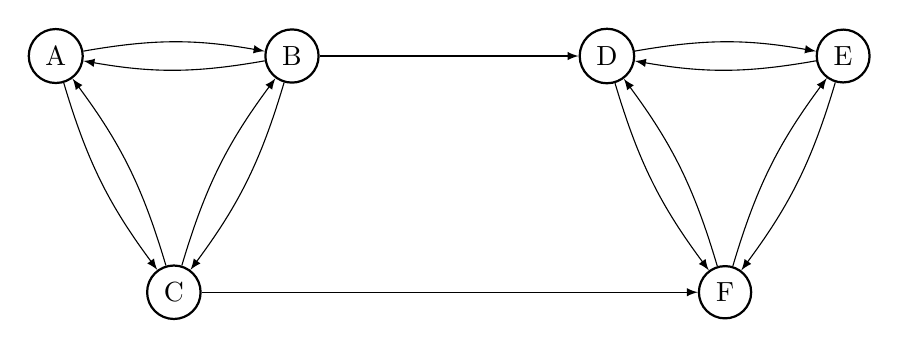
\begin{tikzpicture}[every node/.style={circle,thick,draw}]
        \tikzset{edge/.style = {->,> = latex}}
        \node (A) at (0,3) {A};
        \node (B) at (3,3) {B};
        \node (C) at (1.5,0) {C};
        
        \node (D) at (7,3) {D};
        \node (E) at (10,3) {E};
        \node (F) at (8.5,0) {F};
        
        \draw[edge] (A) to[bend left=10] (B);
        \draw[edge] (A) to[bend right=10] (C);
        \draw[edge] (B) to[bend left=10] (A);
        \draw[edge] (B) to[bend left=10] (C);
        \draw[edge] (C) to[bend right=10] (A);
        \draw[edge] (C) to[bend left=10] (B);
        
        \draw[edge] (D) to[bend left=10] (E);
        \draw[edge] (D) to[bend right=10] (F);
        \draw[edge] (E) to[bend left=10] (D);
        \draw[edge] (E) to[bend left=10] (F);
        \draw[edge] (F) to[bend right=10] (D);
        \draw[edge] (F) to[bend left=10] (E);
        
        \draw[edge] (B) to (D);
        \draw[edge] (C) to (F);
\end{tikzpicture} 
    \caption{Dois grafos K3 ligados por duas arestas}
    \label{fig:my_label}
\end{figure}

\begin{algorithm}[H]
\caption{Gerar dois K-N grafos ligados por duas arestas}
\begin{algorithmic}[1] 
    \REQUIRE $n > 0$
    \STATE $edges_{k1} \leftarrow getCompleteGraph(0, n / 2)$
    \STATE $edges_{k2} \leftarrow getCompleteGraph((n / 2), n)$
    \STATE $edges \leftarrow edges_{k1}+edges{k2}$
    \STATE $extraEdge_1 \leftarrow (getRandomEdge(0, (n / 2) - 1), getRandomEdge((n / 2), n - 1))$ 
    \STATE $extraEdge_2 \leftarrow (getRandomEdge(0, (n / 2) - 1), getRandomEdge((n / 2), n - 1))$
    \WHILE{$extraEdge_1 = extraEdge_2$}
        \STATE $extraEdge_1 \leftarrow (getRandomEdge(0, (n / 2) - 1), getRandomEdge((n / 2), n - 1))$ 
        \STATE $extraEdge_2 \leftarrow (getRandomEdge(0, (n / 2) - 1), getRandomEdge((n / 2), n - 1))$
    \ENDWHILE
    \STATE $edges \mathrel{{+}{=}} extraEdge_1$
    \STATE $edges \mathrel{{+}{=}} extraEdge_2$        
    \RETURN $edges$

\end{algorithmic}
\end{algorithm}

\begin{algorithm}[H]
\caption{Gerar K-N grafo}
\begin{algorithmic}[1]
\REQUIRE $(start \in \mathbb{Z}) \land (end \in \mathbb{Z} \land start \neq end)$
\STATE $edges \leftarrow NULL$
\FOR{$i \leftarrow start, end$}
\FOR{$j \leftarrow start, end$}
\IF{$i \neq j \space \land (i,j) \notin  \space edges \land (j,i) \notin \space edges$}
     \STATE $edges \mathrel{{+}{=}} (i, j)$
      \STATE $edges \mathrel{{+}{=}} (j, i)$
\ENDIF
\ENDFOR
\ENDFOR
\RETURN $edges$
\end{algorithmic}
\end{algorithm}

\subsection{Tempo de execução}

Para os resultados dos testes, achando os determinado tempos de execução para cada situação foi levado em consideração, que os vértices usados como origem e destino seriam respectivamente o primeiro vertice do grafo, ou seja, \textit{0} e o vértice \textit{n - 1}, sendo  \textit{n} a quantidade de vértices presentes no grafo. Para que assim, tenha uma maior quantidade de possibilidades de caminhos disjuntos entre a origem e o destino. Os experimentos foram feitos em uma máquina com as seguintes configurações:

\begin{itemize}
  \item \textbf{Processador}: i7-11390H - 3.4GHz - 2918Mhz - 4 núcleos 
  \item \textbf{Memória}: 16GB - DDR4 - 3200MHz
  \item \textbf{Windows 11}
  \item \textbf{SSD}: 500GB
\end{itemize}

Com isso, uma análise dos gráficos de tempo em relação a quantidade de arestas dos grafos foram feitas, para cada topologia criada no trabalho.

\subsubsection{Topologia 1 - Grafo Circular}

\begin{center}
\begin{table}[ht]
    \centering
    \begin{tabular}{|c | c |}
     \hline
        \multicolumn{2}{|c|}{\textbf{Tempo para execução da topologia 1 (segundos)}} \\
     \hline
         \emph{Quantidade de Vértices} & \emph{Tempo de execução}\\ [0.5ex] 
     \hline
         \emph{10} & 0.000s \\ 
     \hline
         \emph{100} & 0.001s \\
     \hline
         \emph{500} & 0.008s \\
     \hline
         \emph{1000} & 0.010s \\
     \hline
         \emph{10000} & 0.022s\\
     \hline
    \end{tabular}
    \caption{Tempo para execução da topologia 1 (em segundos)}
    \label{tab:tabela_topologia_1}
\end{table}
\end{center}

\begin{figure}[H]
    \centering
    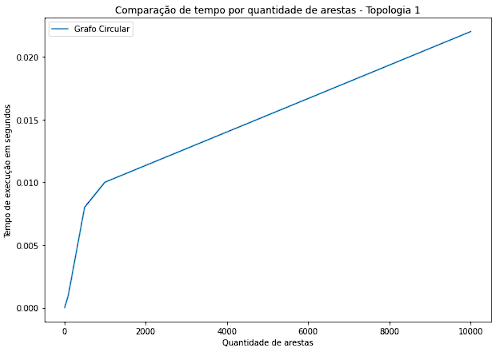
\includegraphics[width=.6\textwidth]{figuras/circular.png}
    \caption{Analise de tempo x quantidade de arestas - Grafo Circular}
    \label{fig:figure20}
\end{figure}

Pode-se observar que no grafo circular o tempo de execução no inicio, onde a quantidade de arestas e menor o tempo de execução acompanha a quantidade de arestas. Com isso, pode-se concluir que ao aumentar o grafo o tempo de execução também aumenta.

\pagebreak

\subsubsection{Topologia 2 - Grafo Simples}

\begin{center}
\begin{table}[ht]
    \centering
    \begin{tabular}{|c | c |}
     \hline
        \multicolumn{2}{|c|}{\textbf{Tempo para execução da topologia 2 (segundos)}} \\
     \hline
         \emph{Quantidade de Vértices} & \emph{Tempo de execução}\\ [0.5ex] 
     \hline
         \emph{10} & 0.000s \\ 
     \hline
         \emph{100} & 0.001s \\
     \hline
         \emph{500} & 1.930s \\
     \hline
         \emph{1000} & 14.130s \\
     \hline
         \emph{10000} & 98.913s \\
     \hline
    \end{tabular}
    \caption{Tempo para execução da topologia 2 (em segundos)}
    \label{tab:tabela_topologia_2}
\end{table}
    
\end{center}

\begin{figure}[H]
    \centering
    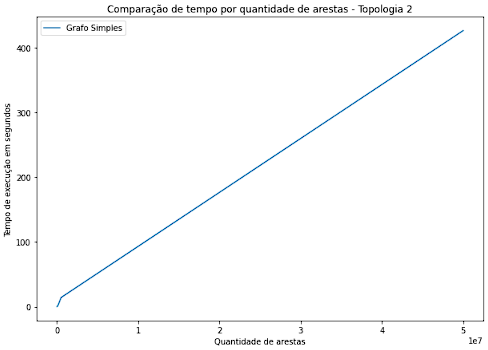
\includegraphics[width=.6\textwidth]{figuras/simples.png}
    \caption{Analise de tempo x quantidade de arestas - Grafo Simples}
    \label{fig:figure30}
\end{figure}

Observa-se que no grafo simples o tempo de execução aumenta linearmente conforme a quantidade de arestas aumenta no grafo, para isso você deve levar em consideração a busca no grafo, que irá continuar sendo executada enquanto o algoritmo encontrar um caminho entre a origem e o destino.

\pagebreak

\subsubsection{Topologia 3 - Grafo Completo}

\begin{center}
\begin{table}[ht]
    \centering
    \begin{tabular}{|c | c |}
     \hline
        \multicolumn{2}{|c|}{\textbf{Tempo para execução da topologia 3 (segundos)}} \\
     \hline
         \emph{Quantidade de Vértices} & \emph{Tempo de execução}\\ [0.5ex] 
     \hline
         \emph{10} & 0.000s \\ 
     \hline
         \emph{100} & 0.002s \\
     \hline
         \emph{500} & 0.014s \\
     \hline
         \emph{1000} & 0.210s \\
     \hline
         \emph{10000} & X \\
     \hline
    \end{tabular}
    \caption{Tempo para execução da topologia 3 (segundos)}
    \label{tab:tabela_topologia_3}
\end{table}

\end{center}

\begin{figure}[H]
    \centering
    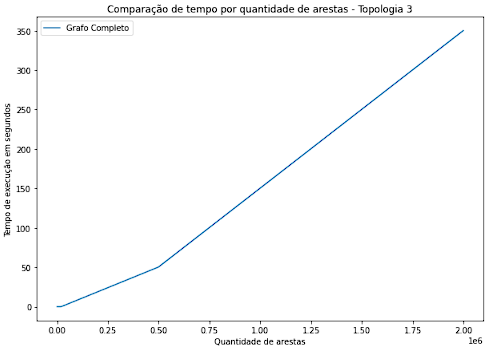
\includegraphics[width=.6\textwidth]{figuras/completo.png}
    \caption{Analise de tempo x quantidade de arestas - Grafo Completo}
    \label{fig:figure40}
\end{figure}

Tendo em vista o grafo completo e sua ligação dos K-N grafos completos por apenas dois caminhos, observa-se que o tempo de execução aumenta conforme a quantidade de arestas presentes no grafo, o que é algo esperado já que os caminhos ficariam mais longos para a busca percorrer, sendo linear o tempo de acordo com a quantidade de arestas.

\subsubsection{Analise tempo por quantidade de vértices}

Para essa analise foi feita a quantidade utilizada a quantidade de vértices presentes no grafo. Com isso, teremos a analise de qual o grafo que tem o maior tempo de execução com certa quantidade de vértices, a mesma quantidade citada no inicio da Seção \ref{sec:results} para todos os testes.

\begin{center}
\begin{table}[ht]
    \centering
    \begin{tabular}{|c | c | c | c|}
     \hline
        \multicolumn{4}{|c|}{\textbf{Tempo para execução por topologia (segundos)}} \\
     \hline
         \emph{Quantidade de Vértices} & \emph{Topologia 1} & \emph{Topologia 2} & \emph{Topologia 3}  \\ [0.5ex] 
     \hline
         \emph{10} & 0.000s & 0.000s  & 0.000s \\ 
     \hline
         \emph{100} & 0.001s & 0.010s & 0.002s \\
     \hline
         \emph{500} & 0.008s & 1.930s & 0.014s \\
     \hline
         \emph{1000} & 0.010s & 14.130s & 0.210s \\
     \hline
         \emph{10000} & 0.022s & 98.913s  & X \\
     \hline
    \end{tabular}
        \caption{Tempo para execução por topologia e quantidade de vértices (em segundos)}
    \label{tab:tabela_topologia_agregado}
\end{table}
\end{center}

\begin{figure}[H]
    \centering
    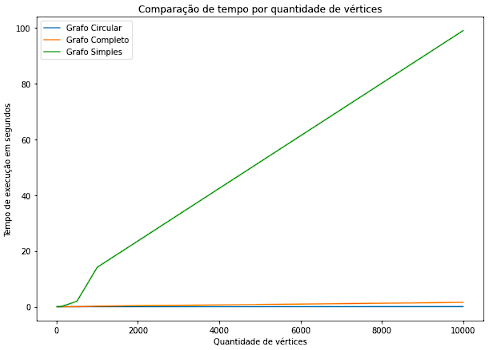
\includegraphics[width=.6\textwidth]{figuras/comparacao.png}
    \caption{Analise de tempo x quantidade de vértices}
    \label{fig:figure50}
\end{figure}

Podemos observar no gráfico da Figura \ref{fig:figure50} que o grafo simples o qual tem uma possibilidade maior de caminhos possui o tempo de execução maior que os demais, já o grafo completo que possui 2 caminhos, possui o tempo de execução maior que o grafo circular que tem apenas 1 caminho presente no grafo. Com isso, pode-se ter certeza que o tempo de execução está diretamente relacionado com a quantidade de arestas e caminhos presentes entre uma origem e o destino.

\section{Conclusão}
Após a aplicação e testes do método podemos concluir que a aplicação da identificação da quantidade máxima de caminhos disjuntos é importante para o cenário de grafos, um exemplo disso é a aplicação desse resultado no \textit{Teorema de de Menger}, onde o número mínimo de vértices que separam A de B é igual ao número máximo de caminhos disjuntos que ligam A a B \cite{SEYMOUR1980293}.

Visto isso, observamos que o algoritmo se baseia em uma busca e os conceitos de caminhos aumentantes onde, após escolher o caminho você deve inverter as arestas. Com isso, observa-se que o algoritmo tem uma implementação simples e obtem resultados muito bons para grafos com poucos caminhos entre uma origem e um destino, porém caso o grafo tenha uma quantidade muito grande de caminhos disjuntos entre um par de vértices o tempo de execução irá aumentar consiferavelmente como mostrado nas analises dos gráficos dos testes presentes na Seção \ref{sec:results}.